\chapter{Introduction and Problem Statement}
\label{ch:intro}

\section{Background and Motivation}
Vietnam features a distinctive elongated geography spanning over 1,650~km from North to South, characterized by diverse topography ranging from rugged northern highlands and central mountain passes to expansive river deltas and an extensive coastline exceeding 3,260~km. Consequently, the country exhibits stark meteorological divergence across its climate sub-regions: subtropical humid conditions with cold winters in the North, intense tropical monsoons accompanied by severe typhoons in the Central region, and distinct wet-and-dry tropical savanna seasons in the South.

Extreme meteorological phenomena---including sudden cloudbursts, severe localized flash floods, high-velocity squall winds, dense mountain fog, and persistent urban inundation---occur with high frequency throughout the year. Adverse weather substantially increases traffic collision frequency, degrades tire-to-surface traction, and reduces driver visibility \cite{andrey2003weather}. In Vietnam, this vulnerability is exceptionally acute due to the unique modal split of the transportation sector: over 72 million registered motorcycles constitute upwards of 85\% of all active vehicular trips. Unlike occupants of enclosed passenger automobiles, two-wheeler riders remain directly exposed to physical weather elements. Heavy precipitation rapidly degrades tire-to-surface traction, strong lateral wind gusts destabilize balance across elevated bridges and coastal causeways, and fog reduces forward sight distance along hazardous mountain passes such as Pha Din, Hai Van, and O Quy Ho.

Despite the profound impact of weather conditions on personal safety and travel reliability, contemporary travelers lack unified digital tools that synthesize continuous spatial meteorology directly into path computation. Bridging the gap between empirical weather observations, geospatial algorithms, and intelligent decision support forms the core motivation of this thesis.

\section{Existing Solutions and Their Limitations}
Modern travelers predominantly rely on two disconnected categories of software applications: commercial geographic navigation platforms and standalone meteorological forecasting services.

\subsection{Commercial Navigation Platforms}
Leading turn-by-turn navigation applications, such as Google Maps, Apple Maps, and open-source OSRM implementations \cite{luxen2011real}, utilize advanced graph contraction and routing algorithms \cite{dijkstra1959note, bast2016route, geisberger2008contraction}. However, their cost functions optimize almost exclusively for physical distance, free-flow travel duration, and historical or crowdsourced traffic congestion. These systems treat the atmosphere as a neutral medium. Meteorological hazards are either ignored entirely or presented as disconnected informational overlays without penalizing high-risk road corridors or providing proactive safety-aware alternatives.

\subsection{Standalone Weather Forecasting Applications}
Conversely, prominent meteorological applications (such as AccuWeather, Windy, and localized hydrometeorological portals) deliver detailed point-based forecasts and radar animations adhering to standard meteorological measurement guidelines \cite{wmo2021guidelines}. Nonetheless, these tools operate in spatial isolation from user navigation. A commuter cannot assess the aggregate weather risk across a 300~km inter-provincial journey traversing multiple climate zones, nor can they determine whether departing 45 minutes later would allow them to bypass a convective storm cell.

\subsection{Generic Generative Artificial Intelligence Tools}
With the advent of Large Language Models (LLMs) \cite{vaswani2017attention, gemini2024flash}, users frequently inquire about travel advice through conversational interfaces. However, unaugmented models suffer from temporal cutoff constraints, lack access to real-time spatial databases, and frequently exhibit hallucinations---generating plausible yet factually incorrect weather claims. Without grounded retrieval and strict function calling protocols \cite{lewis2020retrieval}, conversational models cannot be safely relied upon for mission-critical travel decisions.

\subsection{Comparative Analysis}
Table~\ref{tab:solutions_comparison} provides a structured comparison between existing platforms and the VietForecast system developed in this graduation project.

\begin{table}[H]
\centering
\caption{Feature comparison between existing solutions and VietForecast.}
\label{tab:solutions_comparison}
\footnotesize
\renewcommand{\arraystretch}{0.95}
\begin{tabularx}{\textwidth}{>{\raggedright\arraybackslash}p{5.0cm} *{4}{>{\centering\arraybackslash}X}}
\toprule
Feature Dimension & \makecell{Google\\Maps} & \makecell{Windy /\\AccuWeather} & \makecell{Generic\\LLMs} & \makecell{VietForecast\\(Proposed)} \\
\midrule
Turn-by-turn routing & Yes & No & No & Yes \\
Weather hazard path evaluation & No & No & No & Yes \\
Vehicle-specific risk weighting & No & No & No & Yes \\
Spatial corridor interpolation & No & Partial & No & Yes \\
Real-time verified observations & No & Yes & No & Yes \\
Grounded AI conversation & No & No & Partial & Yes \\
Open-source GIS reproducibility & No & No & No & Yes \\
\bottomrule
\end{tabularx}
\end{table}

\section{Problem Statement and Research Questions}

\subsection{Problem Statement}
Given an origin point $O$, a destination point $D$, a scheduled departure timestamp $t_0$, and a specific vehicle profile $V \in \{\text{Motorcycle}, \text{Automobile}\}$, the problem is to compute a set of alternative navigation paths $\mathcal{P} = \{P_{\text{fastest}}, P_{\text{shortest}}, P_{\text{safer}}\}$ such that each path is evaluated against real-time spatio-temporal weather hazard fields. Specifically, the weather-safer path $P_{\text{safer}}$ must systematically minimize cumulative risk exposure while bounding the acceptable travel time elongation relative to $P_{\text{fastest}}$. Furthermore, the system must enable users to interactively query journey risks through a conversational assistant whose answers are strictly grounded in verifiable observational data.

\subsection{Research Questions}
To address this problem, this research investigates three primary scientific and engineering questions:
\begin{enumerate}[label=RQ\arabic*:]
    \item \textit{Spatial Data Freshness and Normalization:} How can heterogeneous meteorological streams across all 63 provinces in Vietnam be continuously ingested, validated, and normalized into a PostGIS spatial database \cite{postgis2023} with sub-second retrieval latency?
    \item \textit{Multi-Criteria Risk Quantification:} How can multi-modal physical parameters (precipitation rate, gust speed, horizontal visibility, surface wetness, and ambient temperature) be synthesized into an objective, vehicle-differentiated route hazard metric?
    \item \textit{Grounded Conversational Assistance:} How can generative LLM architectures be constrained via deterministic tool calling to drastically suppress hallucinations and generate verifiable, context-aware travel advisories?
\end{enumerate}

\section{Project Objectives and Contributions}

\subsection{Specific Objectives}
The concrete objectives of this graduation project comprise:
\begin{itemize}
    \item Design and implement an automated meteorological pipeline that harvests, validates, and indexes real-time observational data across all 63 provinces of Vietnam.
    \item Develop an extensible, config-driven risk assessment engine that quantifies travel hazard scores tailored distinctly for two-wheelers and passenger cars.
    \item Integrate routing algorithms with geospatial weather surfaces to simultaneously generate Fastest, Shortest, and Weather-Safer routes for trips up to 2,000~km.
    \item Construct a conversational travel assistant powered by Gemini 1.5 with robust function calling against internal geospatial APIs.
    \item Deliver a full-stack, containerized application with sub-second API performance, interactive MapLibre GL visualization \cite{maplibre2024}, and production-ready Redis quota governance.
\end{itemize}

\subsection{Key Contributions}
The key contributions of this thesis are:
\begin{itemize}
    \item An empirical formulation of a composite weather hazard scoring model tailored to Vietnam's road conditions and dominant two-wheeler demographic.
    \item A verifiable spatial-meteorological routing pipeline demonstrating up to 87\% storm avoidance along key Vietnamese transportation corridors.
    \item A production-grade implementation combining modern web technologies (Fastify \cite{fastify2024}, React, TypeScript) and geospatial databases (PostgreSQL/PostGIS) released under reproducible academic standards.
\end{itemize}

\section{Project Scope and Target Audience}

\subsection{Geographical and Operational Scope}
The operational scope encompasses the entire territory of Vietnam, covering all 63 provinces and centrally managed cities, major national expressways (such as the North-South Expressway corridor and National Route 1A), and critical mountainous arterial highways with volatile terrain.

Meteorological data feeds incorporate authentic real-time observation stations and numerical weather predictions standardized under World Meteorological Organization (WMO) protocols. The system supports an actionable forecasting horizon of 72 hours, matching the operational planning window of inter-provincial highway journeys.

\subsection{Target Audience}
The platform addresses the operational requirements of three primary user groups:
\begin{itemize}
    \item Daily commuters and long-distance motorcycle riders: The most vulnerable demographic on Vietnamese roads, exposed directly to intense convective rain, lateral bridge gusts, and dense mountain pass fog.
    \item Passenger car drivers and commercial logistics fleets: Operators requiring advance notice of road inundation, localized storm cells, and flash-flood risks to optimize departure timing and route selection.
    \item Outdoor travel and touring enthusiasts: Independent travelers navigating complex topographic zones who require verifiable en-route weather intelligence.
\end{itemize}

\section{Requirements Analysis and Use Case Modeling}

\subsection{System Requirements Analysis}
Derived from the research questions and operational problem statement, the system requirements are categorized into functional capabilities and non-functional engineering constraints:

\subsubsection{Functional Requirements}
The platform satisfies five core functional requirements:
\begin{itemize}
    \item FR1 (Data Ingestion and Normalization): Ingests periodic weather feeds, maps over 80 external condition codes into canonical classes, and indexes spatial records into PostgreSQL/PostGIS.
    \item FR2 (Vehicle-Specific Hazard Assessment): Evaluates route hazards across six dimensions (rain, wind, temperature, visibility, storms, alerts), applying differentiated weights for motorcycles and cars.
    \item FR3 (Weather-Aware Multi-Path Routing): Discovers three candidate routes (Fastest, Shortest, Safer), segments them at 5--10~km intervals, and projects risk based on ETA over a 72-hour horizon.
    \item FR4 (Grounded Conversational AI): Supports natural Vietnamese queries on route weather, enforcing deterministic tool calling against internal spatial tables to drastically suppress hallucinations.
    \item FR5 (Personalization and Governance): Supports saving favorite itineraries, adjusting risk thresholds, managing RBAC policies, monitoring worker telemetry, and broadcasting emergency bulletins.
\end{itemize}

\subsubsection{Non-Functional Requirements}
The platform complies with four rigorous engineering constraints:
\begin{itemize}
    \item NFR1 (Response Latency): Sub-second API responses for map queries and routing, with Redis caching enabling instant retrieval for repeated requests.
    \item NFR2 (Data Freshness SLA): Surface observations adhere to a 60-minute freshness window, forecast models update daily, and disconnected stations are explicitly flagged.
    \item NFR3 (Security and Session Isolation): Enforces ADR-004 session boundary, withholding Directus tokens from browsers, using opaque HttpOnly cookies, and applying atomic Redis rate limits.
    \item NFR4 (Reliability and Fault Tolerance): Ingestion workers employ circuit breakers and exponential backoff with jitter to maintain service continuity during upstream outages.
\end{itemize}

\subsection{Actor Analysis and Global Use Case Model}
Based on operational requirements and system boundaries, user interactions with VietForecast are categorized into three principal actor roles:
\begin{itemize}
    \item Guest User: Public travelers accessing the web platform anonymously without authentication. Guests can query real-time weather maps across all 63 provinces, execute multi-path weather-safe route computations, and converse with the grounded AI travel assistant for verified meteorological insights.
    \item Registered User: Authenticated travelers who have registered accounts. In addition to inheriting all guest capabilities, registered users can persist trip itineraries, maintain lists of favorite destinations, and configure default vehicle profiles (motorcycle or passenger car) alongside customized weather risk tolerance thresholds.
    \item System Administrator: Privileged operators accessing the Directus Admin Studio to supervise the ingestion worker pipeline, inspect weather observation station records, manage role-based access control (RBAC) policies, and draft and publish localized emergency weather advisories.
\end{itemize}

Figure~\ref{fig:global_use_case_en} illustrates the global use case diagram for the VietForecast platform, delineating system boundaries, actors, and core functional capabilities.

\begin{figure}[H]
\centering
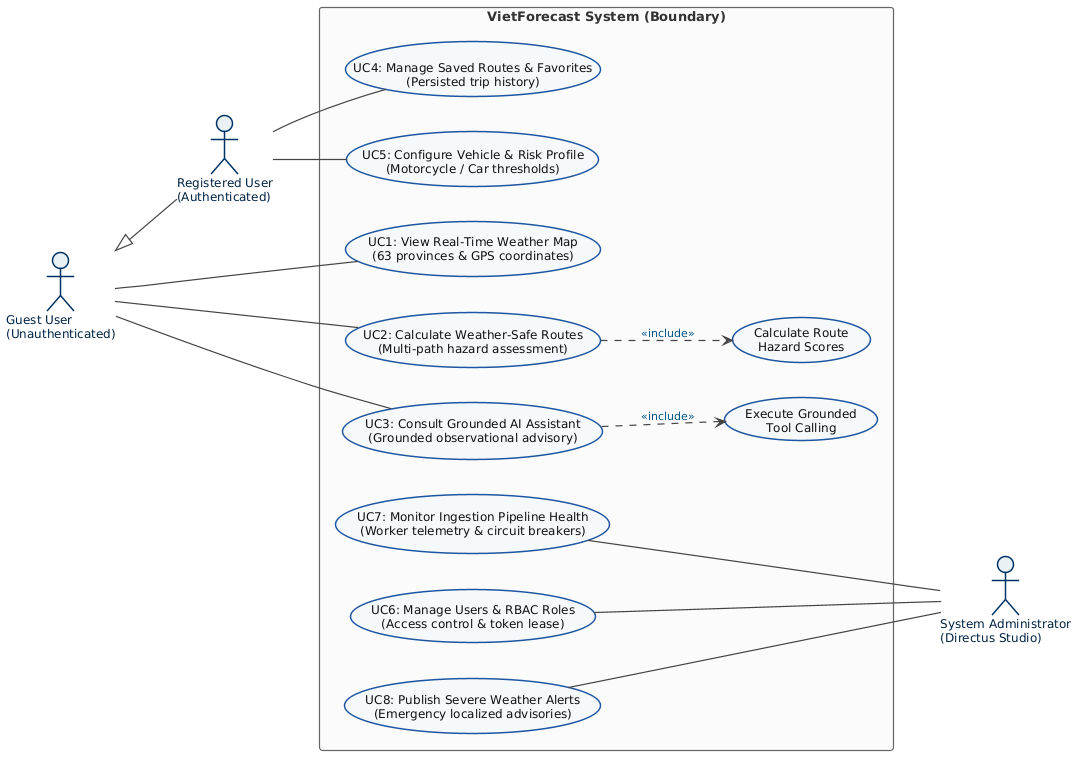
\includegraphics[width=0.95\textwidth]{figures/usecase.png}
\caption{Global use case diagram of the VietForecast platform (UML 2.5 compliant).}
\label{fig:global_use_case_en}
\end{figure}

\subsection{Use Case Summary Specification}
Table~\ref{tab:use_case_summary_en} summarizes the complete catalogue of eight core use cases and two included sub-cases for the VietForecast platform, categorized by primary actors and defining their operational objectives:

\begin{table}[H]
\centering
\small
\caption{Summary specification of VietForecast platform use cases.}
\label{tab:use_case_summary_en}
\begin{tabularx}{\textwidth}{l p{3.4cm} p{2.6cm} X}
\toprule
\textbf{ID} & \textbf{Use Case Name} & \textbf{Primary Actors} & \textbf{Objective and Core Flow} \\
\midrule
UC1 & View Weather Map & Guest User, Registered User & Renders real-time geospatial weather overlays across all 63 Vietnamese provinces or current GPS coordinates. \\
\midrule
UC2 & Calculate Safe Routes & Guest User, Registered User & Discovers three alternative routes, computes multi-hazard risk matrix, and ranks the safest path. Includes hazard scoring sub-case. \\
\midrule
UC3 & Consult AI Assistant & Guest User, Registered User & Provides natural language Vietnamese interaction; executes deterministic tool calling to ground responses in verified station observations. \\
\midrule
UC4 & Manage Saved Routes & Registered User & Persists trip history, preferred travel corridors, and favorite waypoint destinations into the relational database. \\
\midrule
UC5 & Configure Risk Profile & Registered User & Customizes travel vehicle type (motorcycle or car) and configures individualized sensitivity thresholds for weather hazard dimensions. \\
\midrule
UC6 & Manage Users & System Administrator & Manages account lifecycles, configures RBAC policies, and supervises active user sessions via Directus Admin Studio. \\
\midrule
UC7 & Monitor Pipeline Health & System Administrator & Inspects worker process heartbeats, monitors external API circuit breakers, and verifies cache freshness metrics. \\
\midrule
UC8 & Publish Weather Alerts & System Administrator & Drafts, approves, and broadcasts emergency localized weather advisories to active users in affected regions. \\
\bottomrule
\end{tabularx}
\end{table}

\subsection{Detailed Use Case Specifications}
To clarify functional requirements and system interaction behaviors, detailed operational specifications for each use case are structured as follows:

\subsubsection{Use Case UC1: View Real-Time Weather Map}
\begin{itemize}
    \item Primary Actors: Guest User, Registered User.
    \item Preconditions: Client device has active Internet connectivity; Fastify API Gateway and MapLibre GL map engine are operational.
    \item Postconditions: Interactive map correctly displays thematic meteorological layers (temperature, precipitation, wind, visibility) at selected coordinates.
    \item Main Flow of Events:
    \begin{enumerate}
        \item The user accesses the web application or triggers the GPS geolocation button.
        \item The frontend dispatches a spatial query request to the API Gateway.
        \item The system checks cache freshness in Redis; if valid, cached GeoJSON is returned immediately; otherwise, the nearest observation station is queried from PostgreSQL/PostGIS.
        \item The UI renders detailed meteorological metrics alongside intuitive thematic heatmap overlays on the vector basemap.
    \end{enumerate}
    \item Alternative / Exception Flow: If GPS permission is denied, the system defaults to the geographical center of Hanoi and prompts an informative notification.
\end{itemize}

\subsubsection{Use Case UC2: Calculate Weather-Safe Routes}
\begin{itemize}
    \item Primary Actors: Guest User, Registered User.
    \item Dependency: Includes ($\ll$include$\gg$) the Calculate Route Hazard Scores use case.
    \item Preconditions: User provides valid origin and destination coordinates within Vietnam territorial boundaries.
    \item Postconditions: System delivers three distinct route alternatives annotated with composite meteorological risk scores and segment warnings.
    \item Main Flow of Events:
    \begin{enumerate}
        \item The user inputs starting and destination waypoints and selects a vehicle profile (motorcycle or passenger car).
        \item The backend invokes the OSRM routing engine to extract three feasible routes (Fastest, Shortest, Alternative).
        \item The Multi-Path Routing Engine interpolates each route into discrete spatial checkpoints spaced at 5--10 km intervals.
        \item Executes the included Calculate Route Hazard Scores use case: estimates checkpoint arrival times (ETA), correlates spatial forecast points, and computes a multi-dimensional risk score.
        \item The system ranks the safest path (Safer Route) and highlights hazard-prone road segments using color-coded overlays on the map.
    \end{enumerate}
    \item Alternative / Exception Flow: If the upstream OSRM service times out, an exponential backoff retry is executed; if retries fail, a network advisory is displayed to the user.
\end{itemize}

\subsubsection{Use Case UC3: Consult Grounded AI Assistant}
\begin{itemize}
    \item Primary Actors: Guest User, Registered User.
    \item Dependency: Includes ($\ll$include$\gg$) the Execute Grounded Tool Calling use case.
    \item Preconditions: User submits a natural language weather query or navigation inquiry via the chat interface.
    \item Postconditions: The AI assistant delivers a concise, natural language response strictly grounded in verified observation data.
    \item Main Flow of Events:
    \begin{enumerate}
        \item The user enters a natural language prompt (e.g., Is there heavy rainfall on the mountain pass between Hanoi and Sa Pa this afternoon?).
        \item The API Gateway forwards the conversation context to the Google Gemini 1.5 Flash foundation model.
        \item The model detects meteorological intent and emits a structured function call with spatial parameters.
        \item Executes the included Execute Grounded Tool Calling use case: backend retrieves ground-truth observation records from the database and returns JSON data to the model.
        \item The model synthesizes an evidence-backed conversational response, minimizing hallucination risks.
    \end{enumerate}
    \item Alternative / Exception Flow: If the location query cannot be resolved to spatial coordinates, the model prompts the user for geographical clarification.
\end{itemize}

\subsubsection{Use Case UC4: Manage Saved Routes and Favorites}
\begin{itemize}
    \item Primary Actors: Registered User.
    \item Preconditions: User is authenticated with an active session.
    \item Postconditions: Route itinerary or favorite destination is persisted in the PostgreSQL database bound to the user's UUID.
    \item Main Flow of Events:
    \begin{enumerate}
        \item The user clicks the save route button or bookmarks a frequent destination.
        \item The web client transmits the payload with the secure HttpOnly session cookie.
        \item The API Gateway validates user authorization against Directus and inserts records into the database.
        \item The saved route list updates reactively across the user's personal navigation drawer.
    \end{enumerate}
    \item Alternative / Exception Flow: If the session token has expired, the system displays a re-authentication modal while retaining client-side route state.
\end{itemize}

\subsubsection{Use Case UC5: Configure Vehicle and Risk Profile}
\begin{itemize}
    \item Primary Actors: Registered User.
    \item Preconditions: User is authenticated and accesses personal preferences.
    \item Postconditions: Updated risk sensitivity parameters are persisted and applied to future routing computations.
    \item Main Flow of Events:
    \begin{enumerate}
        \item The user navigates to the vehicle and hazard preferences settings.
        \item The user toggles vehicle type (motorcycle or car) and adjusts sensitivity sliders for precipitation, wind gust, or visibility limits.
        \item The user confirms the configuration.
        \item The system updates user metadata, which dynamically shifts weights in subsequent route hazard calculations.
    \end{enumerate}
    \item Alternative / Exception Flow: If parameter values fall outside the normalized 0--100 range, input validation rejects the payload and requests correction.
\end{itemize}

\subsubsection{Use Case UC6: Manage Users and RBAC Roles}
\begin{itemize}
    \item Primary Actors: System Administrator.
    \item Preconditions: Administrator authenticates into the Directus Admin Studio with root privileges.
    \item Postconditions: User account lifecycle states and role assignments are synchronized.
    \item Main Flow of Events:
    \begin{enumerate}
        \item The administrator accesses the user directory in Directus Studio.
        \item Performs administrative tasks: inspecting accounts, revoking access, or updating Role-Based Access Control policies.
        \item The system records all administrative modifications in audit logs for security compliance.
    \end{enumerate}
    \item Alternative / Exception Flow: The system blocks self-demotion or self-deletion attempts to prevent administrative lockouts.
\end{itemize}

\subsubsection{Use Case UC7: Monitor Ingestion Pipeline Health}
\begin{itemize}
    \item Primary Actors: System Administrator.
    \item Preconditions: Administrator accesses the telemetry monitoring dashboard.
    \item Postconditions: Operational telemetry for background integration workers and cache states is displayed.
    \item Main Flow of Events:
    \begin{enumerate}
        \item The administrator inspects worker process heartbeat and telemetry metrics.
        \item The platform reports polling cadence, upstream API latency, circuit breaker state, and Redis cache hit ratios.
        \item If observation freshness exceeds a 60-minute SLA threshold, a high-severity alert is flagged.
    \end{enumerate}
    \item Alternative / Exception Flow: When pipeline failures occur, the administrator can trigger manual ingestion or fallback synchronization.
\end{itemize}

\subsubsection{Use Case UC8: Publish Severe Weather Alerts}
\begin{itemize}
    \item Primary Actors: System Administrator.
    \item Preconditions: Administrator receives official emergency hazard advisories requiring broadcast.
    \item Postconditions: The advisory record is committed and rendered across map interfaces for affected commuters.
    \item Main Flow of Events:
    \begin{enumerate}
        \item The administrator drafts a severe weather bulletin within the Directus Studio.
        \item Sets severity tier (advisory, warning, emergency), hazard type, and geographical bounding polygon.
        \item Approves and publishes the advisory.
        \item The system broadcasts the alert to active map sessions matching the spatial extent.
    \end{enumerate}
    \item Alternative / Exception Flow: If spatial boundaries or required advisory text fields are missing, form submission is blocked until corrected.
\end{itemize}

\section{Conceptual System Context Architecture}
To fulfill the functional and non-functional requirements while preserving system integrity and service reliability, the VietForecast platform is modeled using the C4 architectural paradigm at Level 1 (System Context), as illustrated in Figure~\ref{fig:conceptual_overview_en}. The model explicitly delineates the system boundary, user actor roles, and integrated external cloud services:
\begin{itemize}
    \item Platform Users: Encompasses Commuters and Travelers accessing the platform through responsive web interfaces to inspect live weather maps, compute weather-safe routes, and converse with the grounded AI assistant; alongside System Administrators who oversee operations, monitor pipeline telemetry, and publish localized hazard bulletins via the Directus Admin Studio.
    \item Core Software System (VietForecast Platform): Represents the central computational hub, receiving and dispatching client requests through a high-performance Fastify API Gateway. The platform coordinates the automated ingestion worker pipeline, executes the config-driven multi-dimensional risk engine, evaluates weather-safe navigation alternatives, and hosts conversational LLM interactions grounded in empirical observational records.
    \item External Cloud Services: Encompasses WeatherAPI supplying WMO-standard surface observations and numerical forecasts; OSRM coupled with OpenStreetMap \cite{haklay2008openstreetmap} providing the highway graph and baseline path calculations; and Google Gemini 1.5 Flash operating as the foundation reasoning model constrained via deterministic function calling.
\end{itemize}

\begin{figure}[H]
\centering
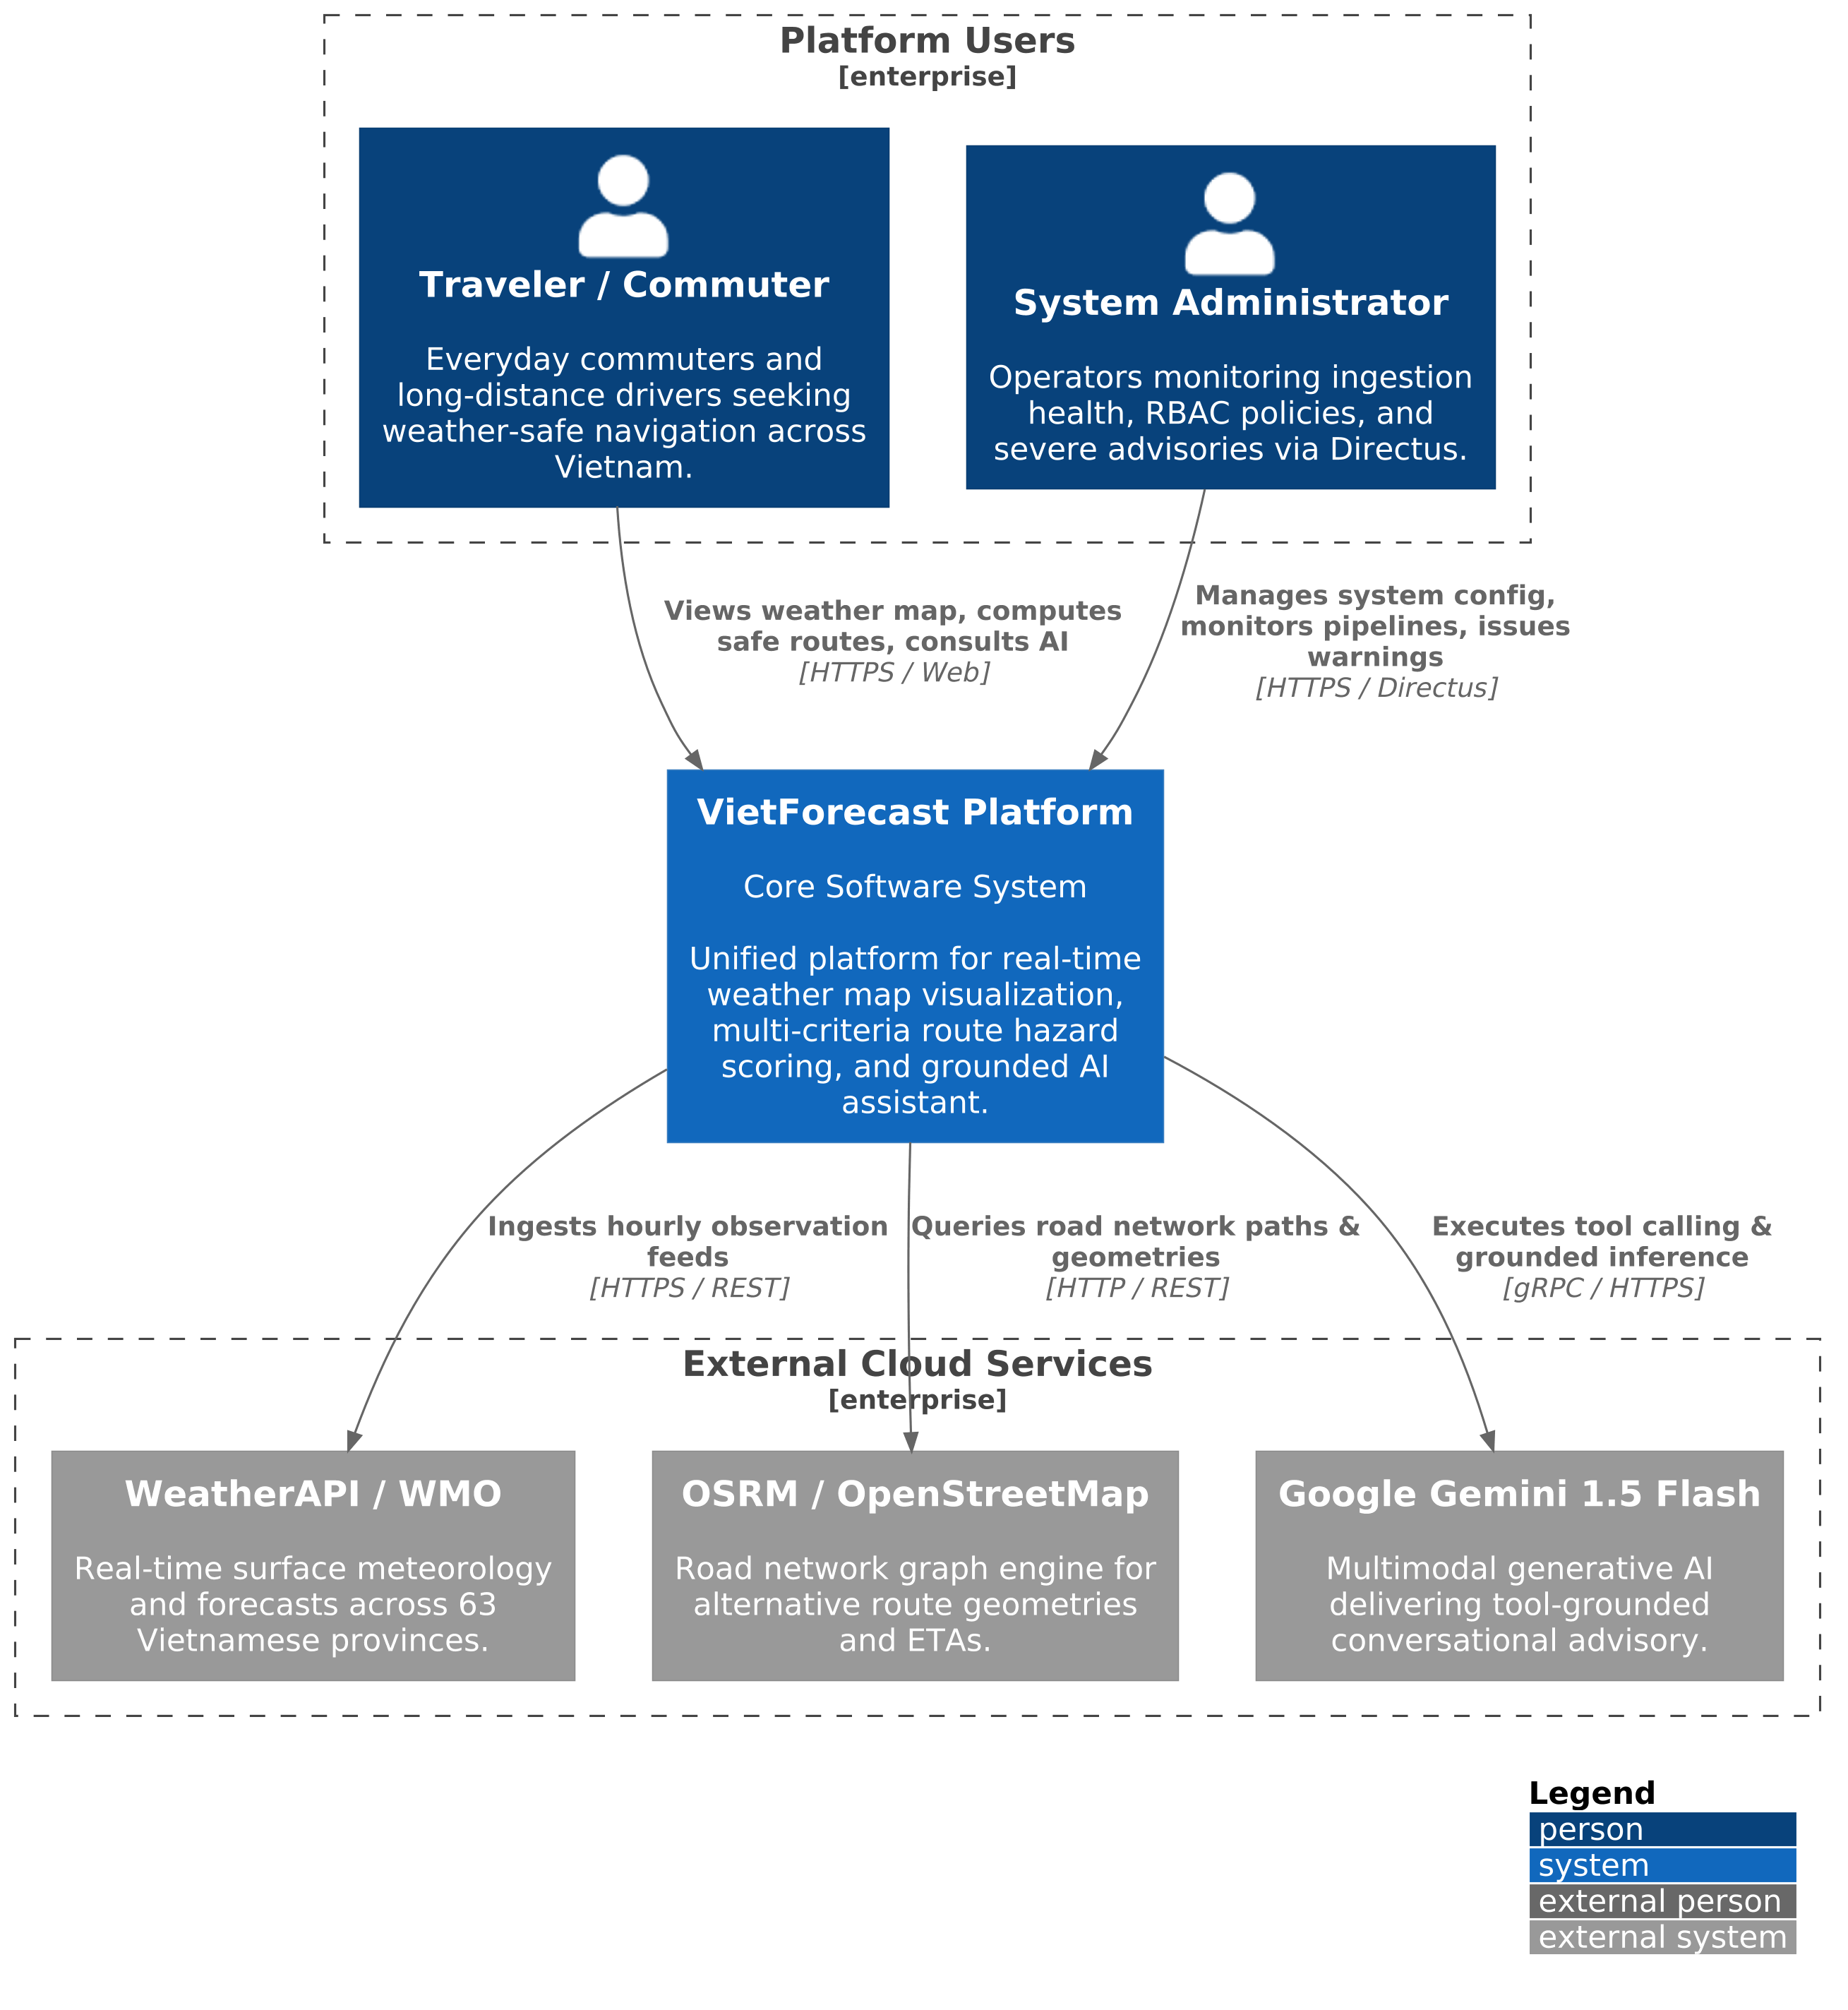
\includegraphics[width=0.92\textwidth]{figures/c4_context.png}
\caption{System context diagram of the VietForecast platform (C4 Model Level 1).}
\label{fig:conceptual_overview_en}
\end{figure}


